\documentclass[letterpaper]{article}

\usepackage[margin=1in]{geometry}
\usepackage{graphicx}
\usepackage{cleveref}


\title{Trundl: An Exploration of Particle Filters}
\author{Jeremy Silver}
\date{\today}
\begin{document}
\maketitle

\abstract{}



\section{Definition}

\subsection{Project Overview}
\label{sec:overview}

For this project, I decided to look at the problem of robot localization and pathfinding under uncertainty. I first started to understand how interesting a problem this could be when I saw a video from Sebastian Thrun's AI for Robotics course at Udacity. The video showed a particle filter localizing a robot in a 


\begin{figure}\label{fig:localization-example}
  \centering
  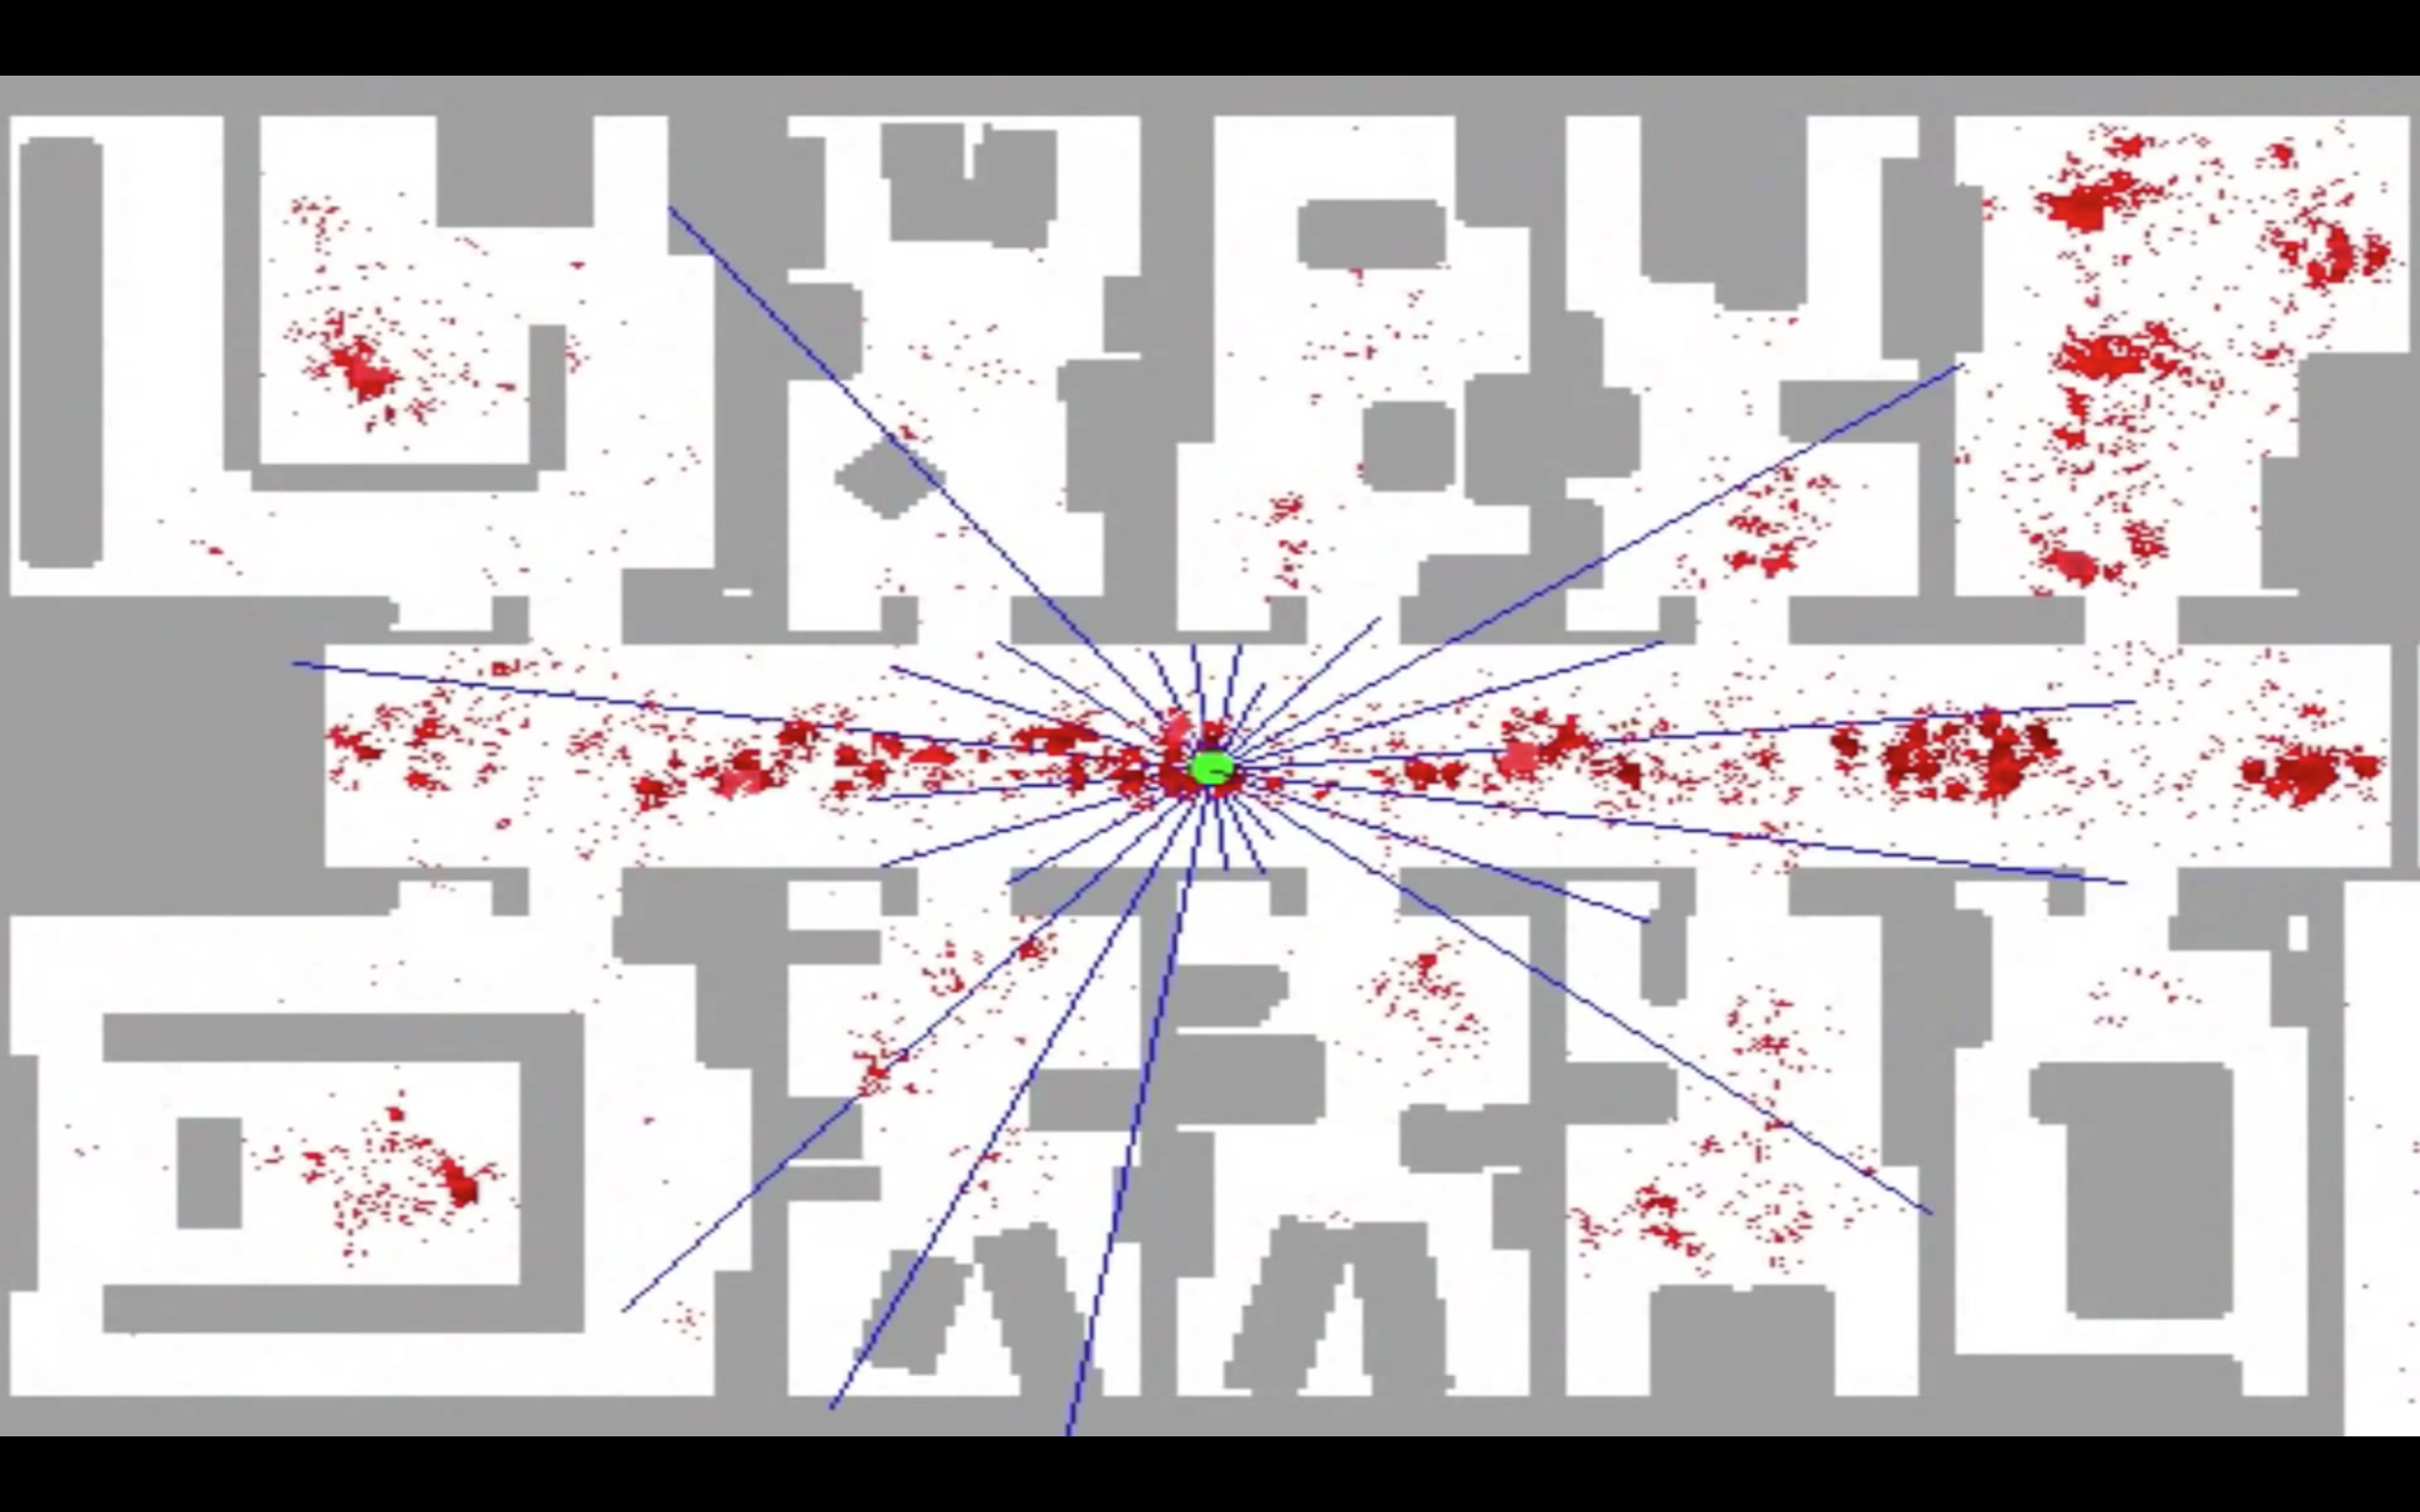
\includegraphics[width=.5\linewidth]{images/localization-example.png}

\caption{Framegrab from \cite{youtube} showing a simulated robot localizing itself within a set of rooms.}

\end{figure}

\subsection{Problem Statement}

The year is 2020, and a young grad student has just passed out in his lab building from exhaustion and overwork. The floor's robot is dispached to revive the student with peptic salve and adrenaline, but someone has moved it since it was last turned on! The robot doesn't know where it is, and to make matters worse, its Mecanum wheels \cite{Diegel02tlale} are sticky, and it's rangefinders are unreliabile! We must help this little bot figure out where on the floor it is, and navigate to the poor grad student without bumping into any walls!

To figure out where the bot is (and keep track of it once we know) we'll use a particle filter. A particle filter proposes many hypothoces about where the bot might be, and as the bot makes measurements, the filter removes hypotoces which are inconsisant with the bots measurements, and duplicates hypotheses that are more likely to be near the bot's actual location.

To determine where the bot should move, we'll divide the floor of the building up into little squares, and then, for every square, compute the proper direction to move to get close to the student, while staying away from the walls.


\subsection{Metrics}

We will consider the project a success if, in repeated runs of this sceneario with random student and bot positions, the bot is able to deliver the salve in time and without crashing 90\% of the time. The time limit will be set to the time required for the bot to travel double the distance that would be required with perfect localization and movement.

These metrics are somewhat arbitrary, but they provide a place to start.

\section{Analysis}

\subsection{Data Exploration}

\subsection{Exploratory Visualization}



\subsection{Algorithms and Techniques}


\subsection{Benchmark}


\section{Methodology}

\subsection{Data Preprocessing}


\subsection{Implementation}




\subsection{Refinement}



\section{Results}


\subsection{Model Evaluation and Validation}


\subsection{Justification}


\section{Conclusion}

\subsection{Free-Form Visualization}

\subsection{Reflection}

\subsection{Improvement}









\bibliography{my_bib}{}
\bibliographystyle{plain}

\end{document}
